\documentclass{article}\usepackage[]{graphicx}\usepackage[]{color}
%% maxwidth is the original width if it is less than linewidth
%% otherwise use linewidth (to make sure the graphics do not exceed the margin)
\makeatletter
\def\maxwidth{ %
  \ifdim\Gin@nat@width>\linewidth
    \linewidth
  \else
    \Gin@nat@width
  \fi
}
\makeatother

\definecolor{fgcolor}{rgb}{0.345, 0.345, 0.345}
\newcommand{\hlnum}[1]{\textcolor[rgb]{0.686,0.059,0.569}{#1}}%
\newcommand{\hlstr}[1]{\textcolor[rgb]{0.192,0.494,0.8}{#1}}%
\newcommand{\hlcom}[1]{\textcolor[rgb]{0.678,0.584,0.686}{\textit{#1}}}%
\newcommand{\hlopt}[1]{\textcolor[rgb]{0,0,0}{#1}}%
\newcommand{\hlstd}[1]{\textcolor[rgb]{0.345,0.345,0.345}{#1}}%
\newcommand{\hlkwa}[1]{\textcolor[rgb]{0.161,0.373,0.58}{\textbf{#1}}}%
\newcommand{\hlkwb}[1]{\textcolor[rgb]{0.69,0.353,0.396}{#1}}%
\newcommand{\hlkwc}[1]{\textcolor[rgb]{0.333,0.667,0.333}{#1}}%
\newcommand{\hlkwd}[1]{\textcolor[rgb]{0.737,0.353,0.396}{\textbf{#1}}}%

\usepackage{framed}
\makeatletter
\newenvironment{kframe}{%
 \def\at@end@of@kframe{}%
 \ifinner\ifhmode%
  \def\at@end@of@kframe{\end{minipage}}%
  \begin{minipage}{\columnwidth}%
 \fi\fi%
 \def\FrameCommand##1{\hskip\@totalleftmargin \hskip-\fboxsep
 \colorbox{shadecolor}{##1}\hskip-\fboxsep
     % There is no \\@totalrightmargin, so:
     \hskip-\linewidth \hskip-\@totalleftmargin \hskip\columnwidth}%
 \MakeFramed {\advance\hsize-\width
   \@totalleftmargin\z@ \linewidth\hsize
   \@setminipage}}%
 {\par\unskip\endMakeFramed%
 \at@end@of@kframe}
\makeatother

\definecolor{shadecolor}{rgb}{.97, .97, .97}
\definecolor{messagecolor}{rgb}{0, 0, 0}
\definecolor{warningcolor}{rgb}{1, 0, 1}
\definecolor{errorcolor}{rgb}{1, 0, 0}
\newenvironment{knitrout}{}{} % an empty environment to be redefined in TeX

\usepackage{alltt}
\usepackage{natbib}
\usepackage{times}

\usepackage{gensymb} % How can I write a ° (degree) symbol in LaTeX?

\newcommand{\BibTeX}{{\sc Bib}\TeX}

\title{Santa Ana Sucker Habitat Evaluation}
\author{C. Flynn, E. Harris-Tyrrell, O. Howie, L. Israel, S. Janssen, \\N. Larson, F. Lyles, W. Nore\~na, V. Sanchez-Jimenez, A. Vacas, D. Wagner,\\ ed. Marc Los Huertos}
\IfFileExists{upquote.sty}{\usepackage{upquote}}{}
\begin{document}

\maketitle

\newpage
\tableofcontents
\newpage

\section{Introduction}

\subsection{Testing Citations}

\LaTeX{} is a typesetting system developed by Leslie
 \citet{lamport94}.  It builds on foundations created by Donald
Knuth's \TeX{} system \citep{knuth79}.  \TeX{} became very popular within
the scientiic community because it was very good at producing
mathematical manuscripts.  It was extremely powerful and provided the
user with exceptional control of the presentation of their documents.
In the 80s, Lamport began developing \LaTeX, which was designed to add a
layer of abstraction on top of \TeX{} which allows the user to focus
more on the document structure, rather than getting too bogged down with
presentation issues.  \LaTeX{} also added extra functionality through
auxiliary programs that can generate bibliographies, tables of contents,
indices, tables, cross-references and figures.

\subsection{Scope of Problem}

The Santa Ana sucker (\emph{Catostomus santaanae}) is a 16 cm fish that lives in the rivers of Southern California.  They have recently been placed on the endangered species list, partially due to their losing over 70 percent of their habitat (FWS 2012). Also, in the 1960s, the habitat of the suckers would range from 10-26\textdegree~C \cite{greenfield70}.  This rise in temperature is most likely due to the extreme industrialization of the stream; much of it runs over concrete, which heats up to extreme temperatures in the sunlight.  A majority of the stream water also comes from discharge from a sewage treatment plant upstream, creating an unhealthy and unnatural environment.  The river discharge is also greatly diminished from what it used to be due to the extreme drought in Southern California.  The river is shallower, slower moving, and has less ice melt coming from the mountains, all of which factor into an increase in temperature. Biological Oxygen Demand (BOD) may also have deviated significantly from typical values in a less disturbed stream. 

As the Santa Ana Sucker's population has declined, the abundance of the red algae (\emph{Cosmopogen aeruginosus}) has risen significantly in the Santa Ana River. This may also be contributing to the sucker's decline, but the environmental variables that control the red algae's distribution in the Santa Ana River are currently not well understood. The direct effect this invasive algae has on \emph{C. santaanae} is also poorly constrained. 

In general, the environmental variables that influence \emph{C. santaanae} populations are poorly understood. Better understanding of water temperature, discharge rates, BOD, and red algae distribution could aid in conservation efforts of this federally endangered fish. 


\subsection{Problem Statement}


This project began with the broad driving question, "How can the Santa Ana sucker be saved?" To that end, we have tried to constrain what environmental variables affect \emph{C. santaanae} distributions. Better understanding of water temperature, discharge rates, BOD, and red algae distribution could aid in conservation efforts of this federally endangered fish.


\subsection{Objectives} 

This experiment explores sevreal aspects of \emph{C. santaanae} habitat and distribution. Using measurments of river water temperature, overhead tree canopy cover, and sediment type we explore the environmental variables of the river and their relationship with the distribution of red algae. Our second goal of this study is to discover whether or not the Santa Ana suckers are coping with this dramatic increase in temperature by moving to cooler sections of the stream throughout the day, by recording video footage of \emph{C. santaanae} movement. 

The report also collected data on the river water temperature to explore relationships between this and other parameters. The following questions were also asked: does the Santa Ana Sucker shift its distribution in the Santa Ana River based on natural temperature changes that occur throughout the day? We believed that if we monitored the relative distribution of the Santa Ana Suckers throughout the day we will see a difference in sucker abundance between an upstream and downstream location in response to changing temperature throughout a 24-hour period. 

Finally, this report aims to determine whether the study of Biological Oxygen Demand (BOD) and water flow velocity are relevant to future conservation research for the endangered Santa Ana sucker \emph{C. santaanae}. The experiment seeks to gather information on the water quality of a section of the Santa Ana River and use this data to help answer the questions: \emph{Are the biochemical oxygen demand (BOD) levels healthy for sucker}, \emph{do differing levels affect the  abundance of individuals in certain sections of the river}, \emph{Are the flow rates in certain sections of the river optimum for sucker populations}, and \emph{do high- or low-flow events affect the number of individuals in the stream?} Because the river is regulated by a water treatment facility, we believe that BOD levels will be very low, increasing with distance from the facility. Because of this, we also expect high dissolved oxygen (DO) content and a high sucker presence. We additionally hypothesize that larger populations of the sucker will concentrate in low-flow areas that are nearby high-flow sections. Through this experiment, we aim to inform Santa Ana sucker conservation efforts and hope to inform action by the nearby water treatment facility. 


<<<<<<< HEAD
=======
The presence of the non-native red algae in the Santa Ana River and the possible relationship it holds with Santa Ana Sucker's decline. In the last five years, the non-native tropical red algae Cosmopogen Aeruginosus has been found in large quantities in the Santa Ana River. Using measurements of river water temperature, overhead tree canopy cover, and sediment type, we explore the connection these aspects of the river and their relationship with the red algae.


Another aspect that this report explored was the Biological Oxygen Demand (BOD) and water flow velocity of the river, to help answer the questions: Are the biochemical oxygen demand (BOD) levels healthy for sucker, do differing levels affect the abundance of individuals in certain sections of the river, Are the flow rates in certain sections of the river optimum for sucker populations, and do high- or low-flow events affect the number of individuals in the stream? Because the river is regulated by a water treatment facility, we believe that BOD levels will be very low, increasing with distance from the facility. Because of this, we also expect high dissolved oxygen (DO) content and a high sucker presence. We additionally hypothesize that larger populations of the sucker will concentrate in low-flow areas that are nearby high-flow sections. Through this experiment, we aim to inform Santa Ana sucker conservation efforts and hope to inform action by the nearby water treatment facility. 


The report also collected data on the river water temperature to explore relationships between this and other parameters. The following questions were also asked: does the Santa Ana Sucker shift its distribution in the Santa Ana River based on natural temperature changes that occur throughout the day? We believe that if we monitor the relative distribution of the Santa Ana Suckers throughout the day we will see a difference in sucker abundance between an upstream and downstream location in response to changing temperature throughout a 24-hour period. 

[needs transition] Does the Santa Ana Sucker shift its distributon in the Santa Ana River based on natural temperature changes that occur throughout the day? We believe that if we monitor the relative distribution of the Santa Ana Suckers throughout the day we will see a difference in sucker abundance between an upstream and downstream location in response to changing temperature throughout a 24-hour period.

>>>>>>> d093b2153263801f35e18898a596e36b42286749
\subsection{Background (Literature Review)}

[FOR NEXT PERSON WHO EDITS: 

WHAT THINGS’ SUSPECTEDSIGNIFICANCE DO WE NEED TO EXPLAIN? 
•	Habitat 
•	Temperature 
•	Red Algae
•	RIX plant
•	The connections between these]


Each of the elements explored in this report was decided as being important to explore based on a review of the following literature:

The range of the fish is of significant interest to efforts for its preservation. The current range of the Santa Ana Sucker differs significantly from its historic distribution in the Los Angeles Basin (Thompson 2010 NO CITATION YET IN R).

Regarding the importance of water temperature to the fish, Moyle postulates that the sucker prefers environments with cool water (Moyle 2002 NO CITATION YET IN R). Again, the temperature of the Santa Ana River has been rising to levels greater than the sucker could stand (CITE). Other types of fish have been known to regulate their body temperatures by moving to different areas in their habitat throughout the day (Matthews Berg Azuma 1994).

We used this source to determine preferred temperature for the Santa Ana Sucker and in general to inform ourselves more about the fish. Little research has been done on specific threats to the Santa Ana Sucker, but the document did point out possible threats arising from hydrological modification and urban development in general. The idea emerged that water coming out of a treatment plant could potentially be a threat under hydrological modification or urban development.


According to Evans et al. (2005 FIND FULL CITATION IN NICOLE AND SOPHIE’S OR CLARE AND WENDY’S GROUP), temporary reduction of flow, such as that which can occur when the treatment plant which now largely supplies the river halts releases of the water which now largely maintains, can significantly reduce the amount of habitat for suckers.[3] Just last month, the Center for Biological Diversity reported that “by halting water releases critical to maintaining surface flows of the Santa Ana River, the Rapid Infiltration and Extraction (RIX) treatment plant is stranding and killing threatened fish.” 

ALGAE: 

For the Santa Ana River sucker habitat, a central threat is the invasive Red Algae that has been spreading with alacrity in areas where the fish are known to be, including the reach below the Rapid Infiltration and Extraction (RIX) Treatment plan (Palenscar).There are concerns that the algae may be one of the contributing factors to the sucker’s decline. For example, one of the important features of the Santa Ana River for the sucker is the presence of coarse substrate, that is, gravel and cobble, as opposed to silt and sand (Thomson et al. 2010, 321 CREATE CITE). The sucker has adapted to feeding on the diatoms that tend to grow on the former. There is also evidence that some of the diatoms on which the sucker feeds may be able to grow on the algae (are epiphytic). 

This may lead to the sucker being in contact with the algae when feeding. If the sucker is ingesting the algae, this may constitute a factor to the Suckers decline. Of course, ingesting the algae is not a necessity to the fish being negatively impacted; the algae may also disrupt the fish’s well-being in unknown ways. 

Some researchers suggest that algae may actually crowd out the diatoms on which, along with algae and detritus, the sucker feeds (Thomson 2010, 322). The presence of the algae in the same area and on the same type of substrate as the fish could indicate competition for resources between the algae and the sh.’ 4 1.3 Objectives


Sadler, K. (1980). Effect of the warm water discharge from a power station on fish populations in the river Trent. Journal Of Applied Ecology, 17(2):349-357.

A power station discharged water that was on average 7 degrees Celsius above normal in the River Trent. This meant that in affected areas, the winter migration was delayed from Sep/Oct to Dec/Jan, while in unaffected areas, migration continued at normal times. Also, below the power station, fish preferred to live further downstream, in terms of diversity and population density. This tells us that fish are able to change their living patterns based on water temperature, and shows that fish were noticeably affected by the temperature change. 


UNNECESSARY?/INFO THAT WAS PREVIOUSLY INCLUDED, JIC:

ON GENERAL HABITAT AUGMENTATIONS: Albertson, L.K., Koenig, L.E., Lewis, B.L., Zeug, S.C., Harrison, L.R., \& Cardinale, B.J. (2012). How Does Restored Habitat for Chinook Salmon (Oncorhynchus Tshawytscha) in the Merced River in California Compare with other Chinook Streams? River Research and Applications, 29(4), 469-482). doi: 10.1002/rra.1604

at Chinook salmon in the Merced river, restoration projects seemed to be failing to prevent the Chinook population from falling. The installation of gravel augmentation in a reconfigured channel seemed to have little impact on the salmon, suggesting that other factors were catalyzing the fall of the species. 
By comparing the restored portion with other portions of the Merced river, food web characteristics and flow discharge seemed to produce the same results on the various life stages of the salmon. However, higher temperatures, less woody debris, and minimal riparian cover seemed to limit populations in the restored portions. 
Restoration efforts are then presented with an added challenge of ensuring that every aspect of the ecosystem is beneficial to the species, which demands more work toward temperature regulation and attempts to restore the river bank. 
To see how the Santa Ana sucker would react to similar conservation efforts would be interesting in discussions in attempting to determine solutions. 

Coulter, D. P., Höök, T. O., Mahapatra, C. T., Guffey, S. C., \& Sepúlveda, M. S. (2015). Fluctuating Water Temperatures Affect Development, Physiological Responses and Cause Sex Reversal in Fathead Minnows. Environmental Science \& Technology, 49(3), 1921-1928. doi:10.1021/es5057159

Human activities can increase water temperature. Water-based organisms are sensitive to temperature change, especially young fish due to limited mobility. Coulter et al. explain how young Flathead Minnows exposed to warmer temperatures underwent a nondirectional sex reversal (Coulter et al 2015). This paper shows us how temperature can greatly affect fish and stress them out. 

TEMP:
Los Huertos, Marc. (2016). Thermal Properties of Water. Environmental Science of Aquatic Systems. 297-308.

The effect of temperature on fish varies greatly depending on other conditions of the lake or river environment of the fish in question.
Heat, temperature, thermal energy, and heat capacity all slightly change how heat is measured in an ecosystem. Water in general has a high heat capacity, which indicates its high specific heat. 

These aquatic systems therefore often retain their heat and are less susceptible to changes in temperature than non-acquatic systems. Inflows/mixing can have an effect on water temperature but it is often hard to detect due to thermal stratification mixing, seasonal change in temperature profile depth, and small volume inflow in terms of fraction of the lake volume. This chapter sheds light that variations in temperature trigger chemicals dissolving/remaining, tend to raise/lower a fish’s body temperature to the same degree, etc. Temperature impacts many other features of water quality, which will be important to keep in mind going forward with the project.


\subsection{Objectives}
Our goal with this experiment was to find out whether or not temperature was affecting the population and/or livelihood of the Santa Ana Sucker in the Santa Ana River.

Our goal is to obtain footage clearly showing the density of Santa Ana suckers in the different locations at different points in the day.  We hope to get accurate enough footage to count the number of fish in each video, then run an ANOVA test on each location to see if the quantity of fish significantly varies at different times of the day.  If they do, we will be able to conclude that the suckers move throughout the day to find their preferred temperature.

Does the Santa Ana Sucker shift its distribution in the Santa Ana River based on natural temperature changes that occur throughout the day? We believe that if we monitor the relative distribution of the Santa Ana Suckers throughout the day we will see a difference in sucker abundance between an upstream and downstream location in response to changing temperature throughout a 24-hour period.

We hope to measure BOD levels and water flow velocity in different areas of the Santa Ana River and correlate those measurements with FWS data about where the Sucker is living in the river.
\begin{quote}
Our null hypotheses are H0: Water flow velocity and/or BOD levels do not significantly correlate with prevalence of the Santa Ana Sucker.
\end{quote}
\begin{quote}
Our alternative hypotheses are H1: Water flow velocity and/or BOD levels significantly correlate with prevalence of the Santa Ana Sucker.
\end{quote}
If we can reject one or both of our null hypotheses, we can conclude that the study of Biological Oxygen Demand (BOD) and water flow velocity are relevant to future conservation research for the endangered Santa Ana sucker \emph{C. santaanae}.


\section{Methods}

\subsection{Materials and Equipment}
\begin{itemize}
\item 2 Waterproof GoPro Hero 4 Silver cameras with mounts
\item 4 64GB microSD SanDisk memory cards
\item 4 Waterproof Re-Fuel 6-Hour ActionPack Battery for GoPro HERO by DigiPower
\item 2 HOBO Tidbit water temperature data loggers
\item 2 Grey Cinder block cubes open on two parallel sides, ~8in x 8in x 8in, Home Depot
\item 2 Grey Cinder block backs, ~8in x 8in
\item 1 bottle of Original Sticks to Everything Gorilla Glue
\item 4 HOBO Tidbit Water Temperature Data Logger,
\item 1 Optic USB U-4 Base Station with coupler and HOBOware software,
\item 4 Green Garden stakes to hold loggers in stream channel
\item Red flags,
\item Yellow marking tape,
\item Ice Bath for calibrating loggers
\item GPS Spherical Canopy Densiometer
\item 30cm x 30cm PCV Quadrat
\item Analog Thermometer
\item 10 m tapemeasure
\item Field Book Recording material
\item Computer, RStudio Server, Microsoft Exc
\item snorkleing goggles 

\end{itemize}

\subsection{Site Descrition}

We collected our video on-site at the Santa Ana River. As a class we chose to collect data from four points along a small stretch of the river that was easily accessible by car. Because of this, the part of the river we took data from was relatively close to roadways and traffic. 

The specific sites for our project consisted of one upstream location (site 2) and one downstream location (site 4), located roughly one kilometer apart. Site 2 was located just below the Rialto concrete channel and site 4 was a plunge pool. The upstream location was significantly more encumbered with large debris like rocks and branches. The downstream location was smooth and flat, with a bed of pebbles and smaller coarse sediments (Figure \ref{SAR_Image}). 

We evaluated the Santa Ana River between... near Colton, California (Figure \ref{SAR_Image}). 

This data was collected at three reaches in the Rialto portion of the Santa Ana river near Colton, California (Figure \ref{SAR_Image}).

Site 4 was the plunge pool, located the furthest downstream. Site 3 was below the confluence and Site 2 was upstream from the confluence. 


Site 4 (plunge pool): 34* 2’5” N, 117 degrees 21’17” W 
Site 3 (below confluence): 34*2’21” N, 117*21’20” W 
Site 2 (above confluence): 34*2’29” N, 117*21’15” W. 

Each observation contains the following variables: algae percent cover, canopy cover, water temperature, bed composition.  


\begin{figure}
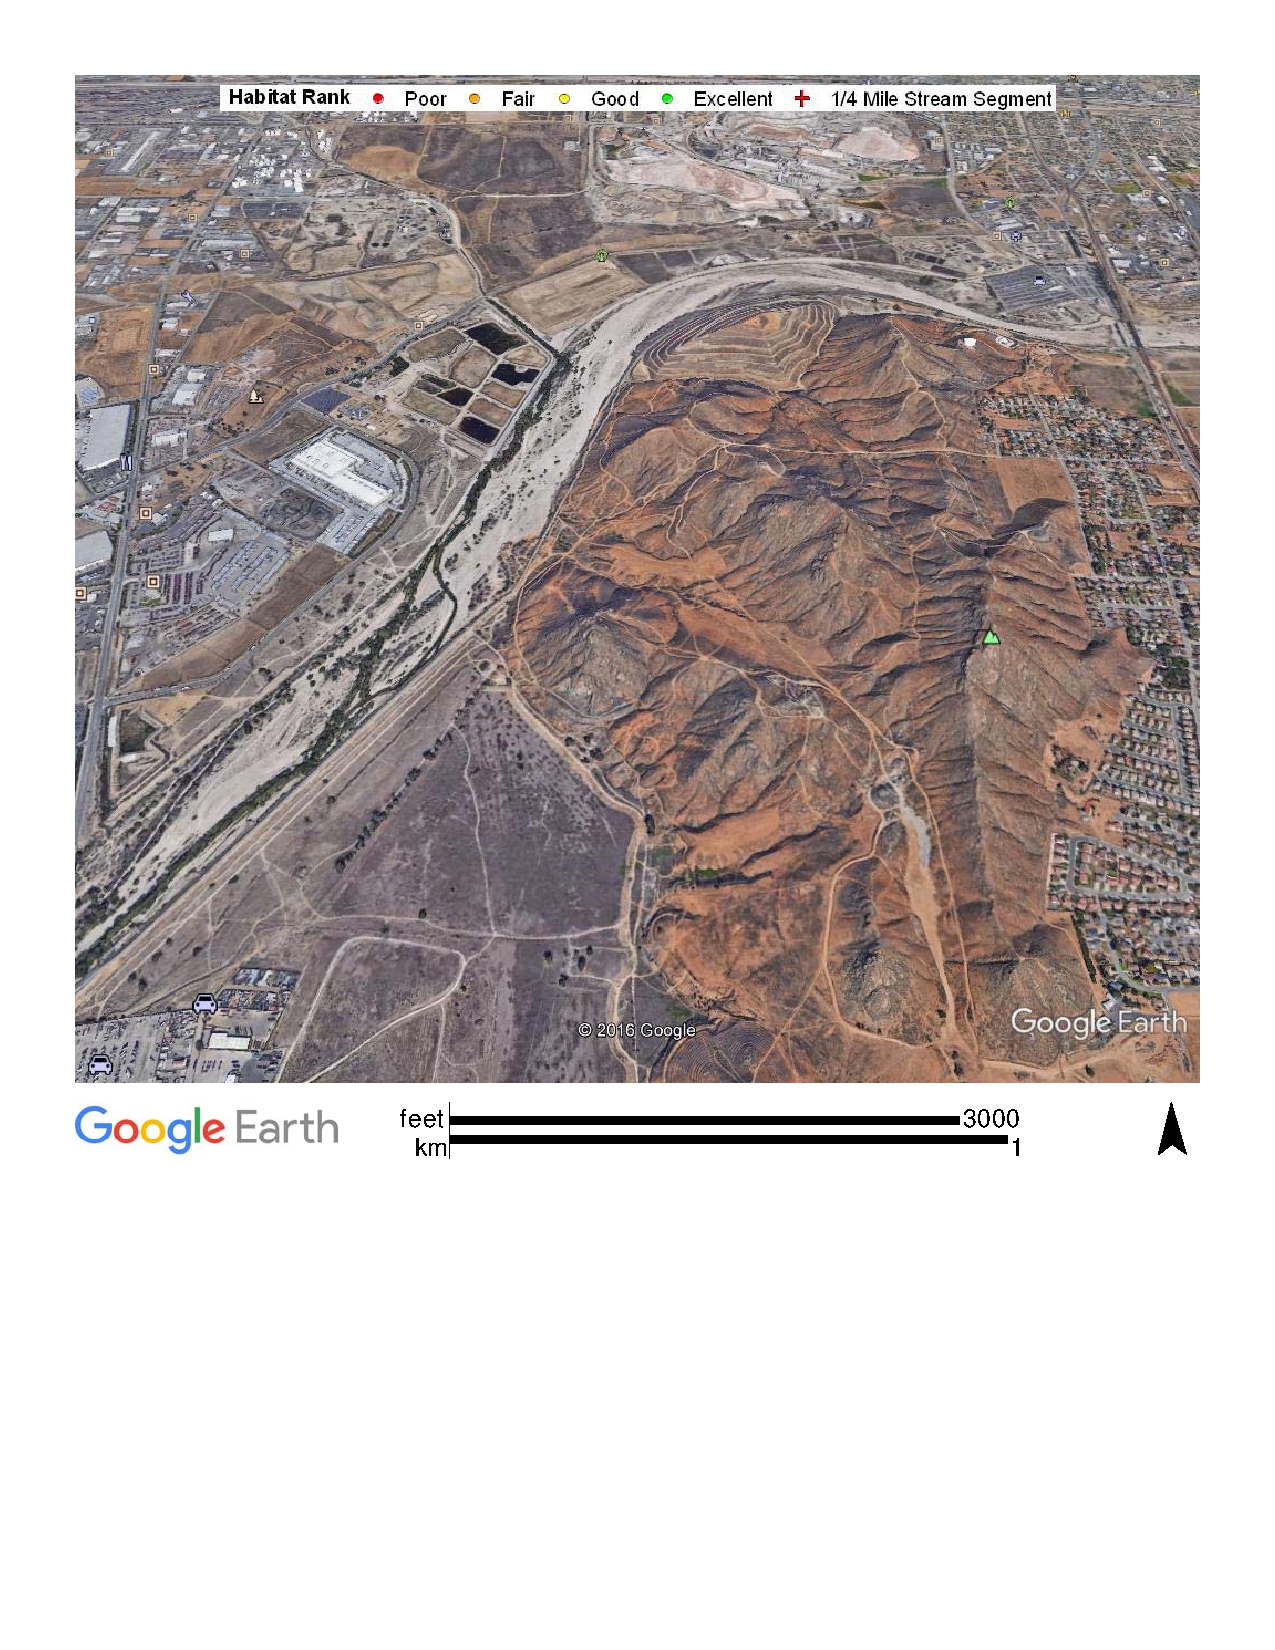
\includegraphics[width=1.00\textwidth]{Figures/SantaAna_SatelliteImage}
\caption{Google Earth --Example of a map. What's wrong with this image?}
\label{SAR_Image}
\end{figure}

\subsection{Habitat Evaluation}

The collection of data on the algae abundance, sediment type, vegetation canopy cover, 
and temperature of the Santa Ana River was done along the section of the river described
in the site description section on September 20th, 2016, from 1pm to 3:30pm.

9 measurements of each parameter were taken at Sites 4, 3, and 2, for a total of 27 measurements. 
At each site, beginning at Site 4, the following procedures were followed: 

1)A spot was chosen along the right bank. Each of the parameters were then measured.

2)For estimating algae abundance, we placed the 30  x 30 cm quadrat above the river bed and estimated
the percent that was covered by algae to the nearest 10 percent.

3)The sediment type of the site was characterized as either fine or coarse based on the grain size of the 30x30cm section of stream bed covered by the quadrat as either fine or coarse. Coarse substrate was classified as anything larger than pebbles or sand, that is, larger than 6.5cm. If more than half of the area covered by the quadrat was coarse substrate, or fine substrate, the area was characterized as such respectively.

4)Canopy cover was measured from the same position as the algae by holding spherical canopy densiometer above water at elbow’s length. Based on how many of the 15 intersections on the densiometer reflected overhead canopy, cover was then quantified on a 0-15 scale, 0 being the no canopy cover and 15 being full cover.

5)To measure temperature, we submerged the analog thermometer underwater and recorded the temperature in degrees Celsius.

6)Qualitative aspects of the river, such as presence of a pool or of logs, were also noted at each measurement spot.

7)Each measurement was then also taken at the middle of the river and the left bank of the cross-section. 

8)Steps 1)-7) Were repeated at two cross-sections between 0 and 10 meters downstream both chosen using a random number generator for a total of 3 cross-sections along a possible total length of 20 meters, and 3 measurements at each cross-section, for a total of 9 measurements per site. 


Steps 1)-8) were repeated at each Site, moving upstream from 4 to 2, for a total of 27 measurements of each parameter.



At each of the corresponding water sample collection sites, water velocity was also measured using a SonTek FlowTracker Handheld Advanced probe, which emits sonar waves at a certain depth in the water column, and based on the feedback (20 pings) gives a velocity reading. Ideally, multiple readings would be taken at each site, after the probe is placed on a flat section of the riverbed where water appears to be flowing net in the same direction. 

\subsection{Videography}

We acquired all the necessary equipment for an underwater filming project, keeping in mind the length of time we wanted to keep our cameras underwater. We chose the GoPro Hero 4 Silver because of its battery life and recording time. We also considered safety and theft prevention for the cameras, and for this reason decided to mount the cameras in cube-shaped cinderblock structures with one open side that we constructed ourselves. In the lab, we set up all the equipment, built the cinderblock structures, and prepared everything for the field. Once in the field, we selected appropriate data sites, set up our cameras, and placed them at certain specific times of the day. More detailed information on these processes can be found in the following sections.

\subsection{Temperature Loggers}
We will obtain four HOBO Tidbit water temperature Data Loggers to set up at the Rialto Channel at Agua Mansa (site 4), another at the point where the other discharge site meets the river (site 2), another just above that site (site 3), and a fourth in the pool where Suckers have previously been observed (site 1). Before going to the river, we programmed the loggers via our base station and the HOBOware software to collect water temperature data every 15 minutes. In order to start the data process, we put each logger into the coupler and pushed the level til the light was flashing. We then put them in the river by looping a garden stake through one, sticking it into the substrate, and securing it with rocks. We then put yellow marking tape on plants nearby and red flags along the bank to show where we left the main path. We repeated this for each site, making sure the loggers were secure and fairly hidden. After seven nights (for site 3) and eleven nights (for the other sites), we returned to the river and collected the loggers. In the lab, using the software, we loaded our data and transferred it to RStudio. Later, to calibrate the loggers, we put them in an ice bath for 6 minutes to ensure that the temperature settled around zero and each logger was measuring to the same temperature with the same accuracy.

\subsection{BOD Methods}

Approximately 1L of source river water was collected at each of two sites, one upstream location closer to the wastewater discharge facility, and one downstream location (fig. 1). Ideally, these would be transported to the laboratory for analysis within four hours.

Ideally within the same day of collection, water samples were analyzed for initial dissolved oxygen content and prepared for 5-day incubation.  
\begin{itemize}
  \item Three different dilutions were used for each of two sites, with source water volumes of 25, 50, and 100 mL. 
  \item A seed suspension was prepared using PolySeed Seed Innoculum, and 4 mL of the solution was added to each 300 mL sample bottle. This solution was also used to create four seed blanks with seed volumes 15, 20, 25, and 30 mL.
  \item Nitrification inhibitor was created by dissolving 2.0 g allylthiourea (ATU, C4H8N2S) in 1 L distilled water. 0.3 mL of the ATU solution was added to each source water sample, as well as to all seeded samples. 
  \item A glucose-glutamic acid (GGA) solution was prepared by dissolving 150 mg each of dry glucose and glutamic acid in 1 L of distilled water, and was added to each of the four seed blanks, as well as the six source water samples. Three GGA blanks were also created with 6 mL of GGA solution in incubation bottles. 
  \item Dilution water was created using 1 mL each phosphate buffer (8.5 g KH2PO4, 21.75 g K2HPO4, 33.4 g Na2HPO*7H2O, and 1.7 g NH4Cl dissolved in 1 L distilled water), Magnesium sulfate solution (4.5 g MgSO4*7H2O dissolved in 200 mL distilled water), Calcium chloride solution (5.5 g CaCl2 dissolved in 200 mL distilled water), and Ferric chloride solution (0.05 g FeCl3*6H2O dissolved in 200 mL distilled water), and added to the six source water samples, four GGA blanks, and three seeded blanks. Three dilution water blanks were also created using the same procedure diluted to 300 mL.
\end{itemize}
Initial DO readings were to be taken on all blanks and samples using a Thermo Scientific DO Probe with auto-spinning functionality. The bottles were then incubated in a dark area for 5 days, and DO readings were again taken.  

Note that *Temp\_x* entries were borrowed with permission from Sophie and Nicole's dataset. We also created a "Site\_New" field so that our naming conventions whould be consistant with other teams. We then used rstudio to generate the following descriptive statisitcs:  
linear regression of temperature range vs algae abundance
linear regression of canopy cover vs algae abundance
ANOVA of bed composition vs. algae abundance
ANOVA of site location vs. algae abundance
For each of these statistical comparisons, we tested whether we could reject the null hypothesis, and if yes, discuss the implications of those findings. Our results are summarized in the following section. 

\subsubsection*{Quality Control Checks}
Using the seed blanks, glucose-glutamic acid blanks, and dilution water blanks, quality control checks were performed prior to data collection. 
\begin{itemize}
  \item Minimum DO Depletion--Viable samples must have min. DO depletion of 2.0mg/L, and residual DO of at least 1.0mg/L.
  \item Glucose-Glutamic Acid Check--The resulting average BOD for the 3 GGA blanks (after correction for dilution and seeding) must be 198+/- 30.5mg/L.
  \item Dilution water check--DO uptake after incubation must not be more than 0.20mg/L and preferably not more than 0.10 (before seed corrections). 
  \subitem Dilution Water--If dilution water blank exceeds 0.20 mg/L, clearly identify samples in data.
  \item Seed control--Calculate Seed Control Factor (SCF) using [(D1-D2)*f], where
  \subitem D1= initial DO of seed control, mg/L
  \subitem D2= final DO after indubation, mg/L,
  \subitem f= (vol. seed in diluted sample)/(vol. seed in seed control)
\end{itemize}

\subsubsection*{BOD5}
BOD5 was calculated for viable samples according to Standard Methods for the Examination of Water and Wastewater, using the equation 
BOD5, mg/L= ((D1-D2)-(S)Vs)/P, where 


D1= initial DO, mg/L

D2= final DO after incubation, mg/L


\subsection{Statistical Methods}

After conducting our fieldwork, we will enter our data in rstudio. We will produce linear regressions of temperature vs algae abundance. We will producelinear regressions of canopy cover vs algae abundance. We will produce linear regressions of canopy cover vs temperature. We will create ANOVA or t-tests of bed composition vs. algae abundance. We will then analyze our data and write a project report 4-5 pages long with pictures and figures. We should hopefully be able to draw conclusions about canopy cover, temperature, and stream bed compositions effect on algae abundance. In qualitative terms, we will synthesize our results with the fish videography team and state whether our observed relationship between stream conditions and algae abundance matches the frequency of their fish observations.
The following code was used to generate summary statisitics. 


\subsection{Statistical Methods}

We ran an ANOVA test where time period was the categorical independent variable and number of fish was the continuous dependent variable.  We weren’t able to run the test for location 2 because there were too few fish seen to draw any conclusions.  We also couldn’t test the effect of location on number of fish, because the conditions were too different between the upstream and downstream locations to compare.

\section{Results}

\begin{knitrout}
\definecolor{shadecolor}{rgb}{0.969, 0.969, 0.969}\color{fgcolor}\begin{kframe}
\begin{alltt}
\hlstd{updateddata}\hlkwb{=} \hlstr{"/home/CAMPUS/fcl02013/Santa-Ana-Sucker-Recovery/Data/Data_TUES_1/updatedtemps.csv"}
\hlstd{importupdated}\hlkwb{=}\hlkwd{read.csv}\hlstd{(updateddata)}
\end{alltt}
\end{kframe}
\end{knitrout}


The tempeature data suggests... (Figure \ref{Temp}).

\begin{figure}
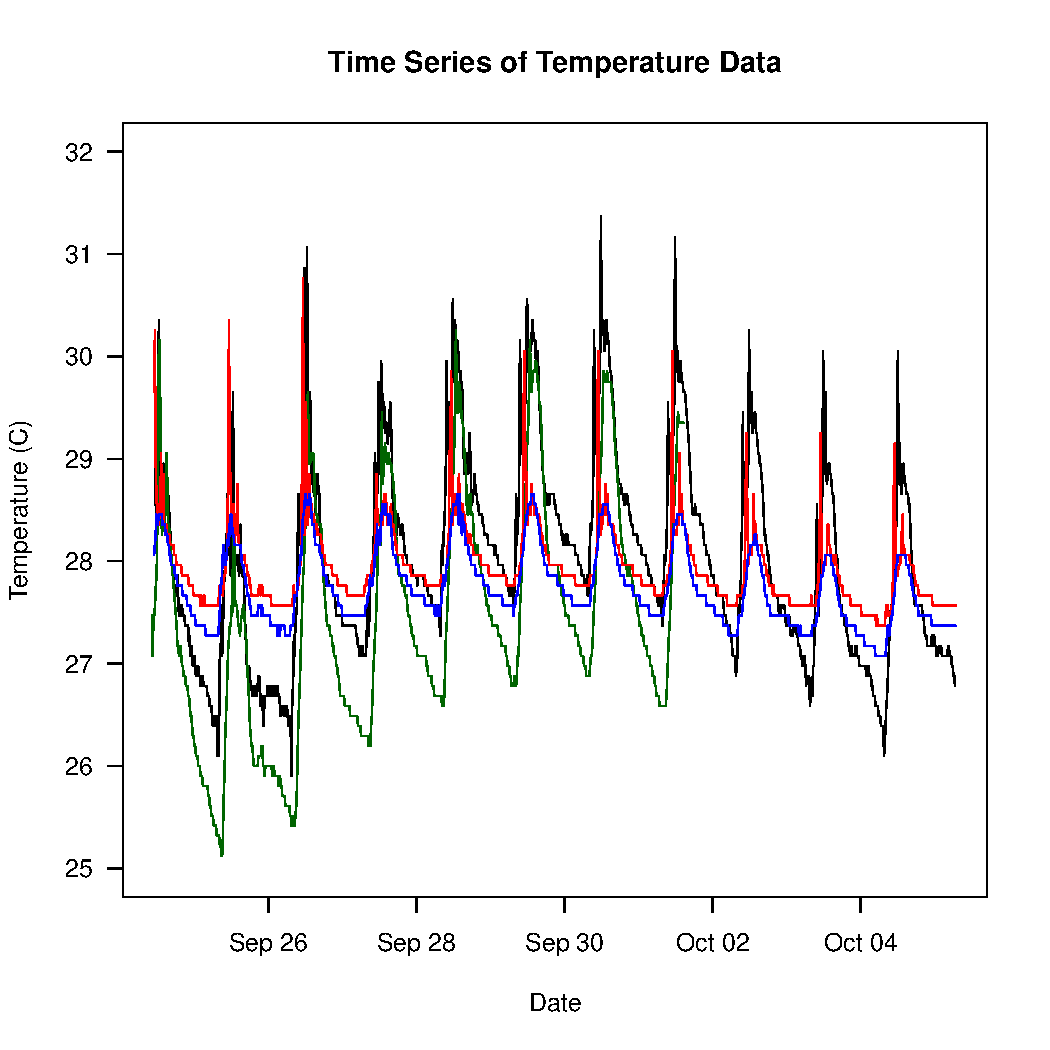
\includegraphics{Figures/Temp}
\caption{Temperature time...}
\label{Temp}
\end{figure}

The Seed Control Factor was calculated for the four seed blanks, and the slope of the resulting values and the corresponding seed concentrations was determined. Analysis of the data using quality control parameters indicated that two source water samples met minimum DO depletion standards. Our BOD5 calculations on these data yielded the values:

upstream BOD5= 22.069 mg/L 

Downstream BOD5= 27.3493 mg/L 

The temperature data we collected with an analogue thermometer was too coarse to really be useful, because we took all our measurements in one afternoon and could only take temperature measurments at a resolution of whole degrees celsius. For that reason, we instead used WED1 team's temperature data. The following is a plot of algae abundance as a function of range of temperature (*C) experienced at each site. 

This is describing the figure: (figure \ref{fig:tempalgae})
\begin{figure}
\begin{knitrout}
\definecolor{shadecolor}{rgb}{0.969, 0.969, 0.969}\color{fgcolor}\begin{kframe}
\begin{alltt}
\hlkwd{plot}\hlstd{(importupdated}\hlopt{$}\hlstd{Temp_range,importupdated}\hlopt{$}\hlstd{Algae,} \hlkwc{ylab}\hlstd{=}\hlstr{"Algae Abundance (% cover)"}\hlstd{,}\hlkwc{xlab}\hlstd{=}\hlstr{"Temperature (*C)"}\hlstd{,}\hlkwc{main} \hlstd{=}\hlstr{"Temperature as a predictor of Algae Abundance"}\hlstd{,}\hlkwc{las}\hlstd{=}\hlnum{1}\hlstd{)}
\hlkwd{abline}\hlstd{(}\hlkwd{lm}\hlstd{(Algae}\hlopt{~}\hlstd{Temp_range,importupdated))}
\end{alltt}
\end{kframe}
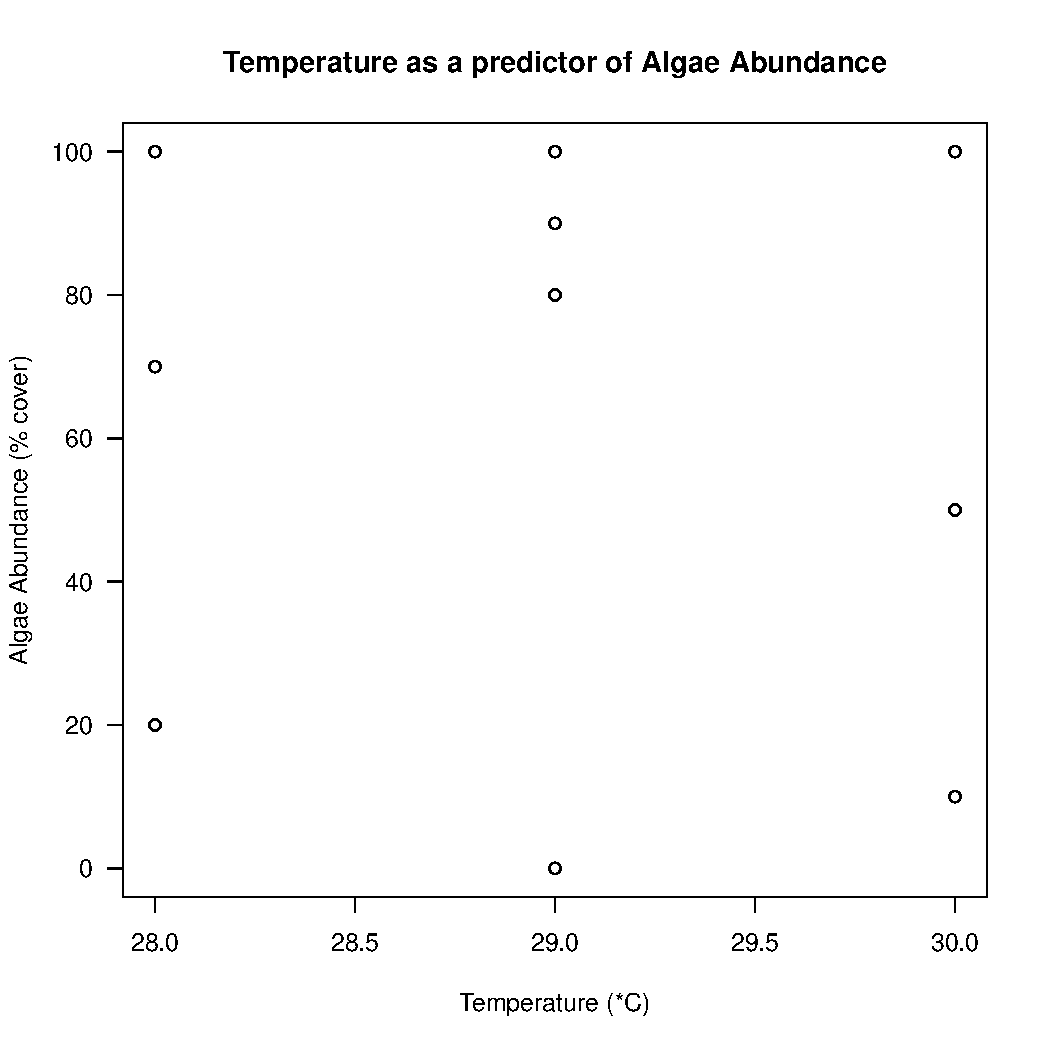
\includegraphics[width=\maxwidth]{figure/unnamed-chunk-2-1} 

\end{knitrout}
\caption{Ths is caption}
\label{fig:tempalgae}
\end{figure}
<<<<<<< HEAD
While using our absolute temperature data as a predictor of algae abundance yielded p-value: 0.446 (cannot reject null hypothesis), using the other teams's temperature d range data yilded the much better p-value of 3.49e-05. There is a strong nonrandom relationship between the range of temperatures a site experiences and the abundance of algae. However, with an Adjusted R-squared of only 0.4826, there are clearly other important variables at work as well. We find that higher variation in water temperatures generally coorelates to higher algae abundance. 

\begin{knitrout}
\definecolor{shadecolor}{rgb}{0.969, 0.969, 0.969}\color{fgcolor}\begin{kframe}
\begin{alltt}
\hlkwd{plot}\hlstd{(importupdated}\hlopt{$}\hlstd{Canopy,importupdated}\hlopt{$}\hlstd{Algae,} \hlkwc{ylab}\hlstd{=}\hlstr{"Algae Abundance (% cover)"}\hlstd{,}\hlkwc{xlab}\hlstd{=}\hlstr{"Canopy Cover Index"}\hlstd{,}\hlkwc{main} \hlstd{=}\hlstr{"Canopy Cover as a predictor of Algae Abundance"}\hlstd{,}\hlkwc{las}\hlstd{=}\hlnum{1}\hlstd{)}
\hlkwd{abline}\hlstd{(}\hlkwd{lm}\hlstd{(Algae}\hlopt{~}\hlstd{Canopy,importupdated))}
\end{alltt}
\end{kframe}
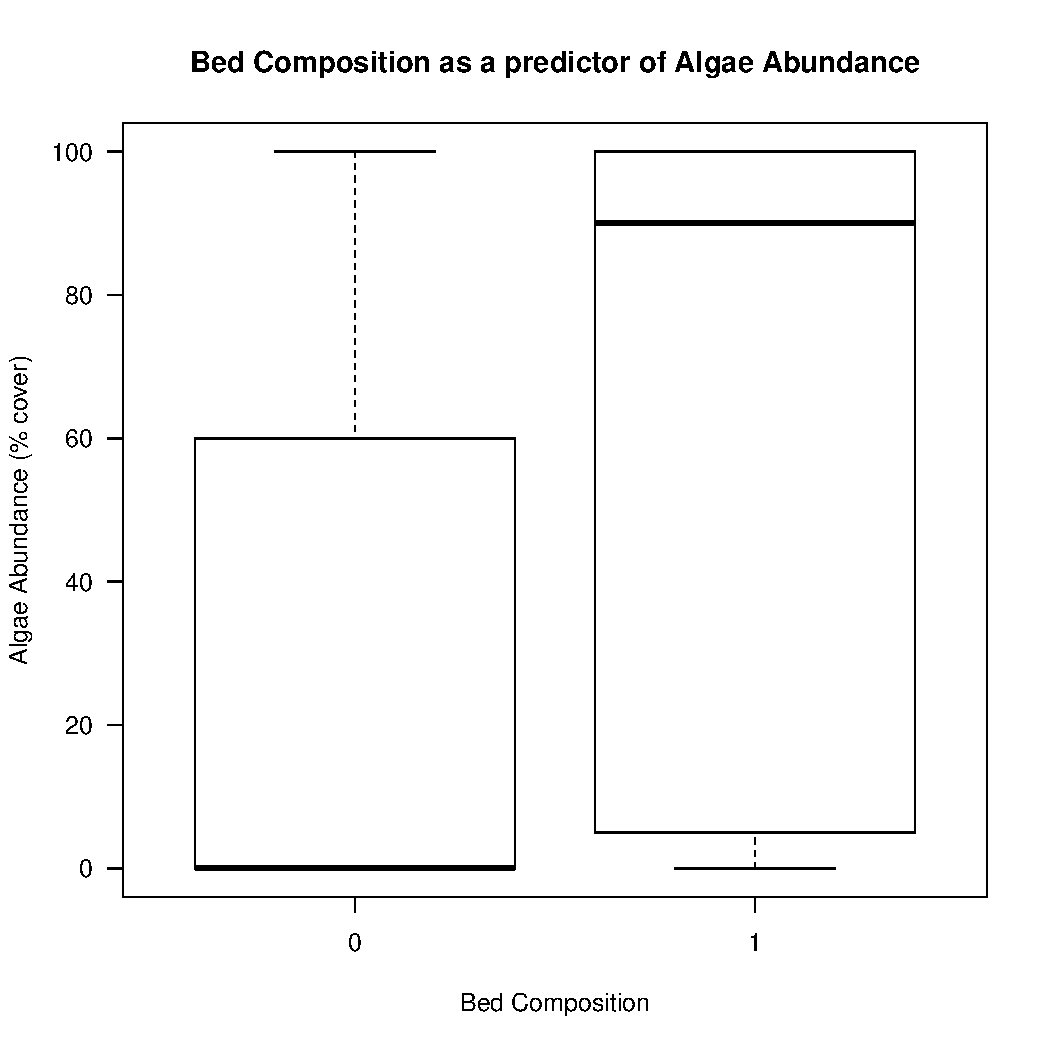
\includegraphics[width=\maxwidth]{figure/unnamed-chunk-3-1} 

\end{knitrout}
Canopy Cover was a very poor predictor of Algae Abnundance, with no predictive value. A linear regression yielded p-value: 0.3339, so we cannot reject the null hypothesis.

\begin{knitrout}
\definecolor{shadecolor}{rgb}{0.969, 0.969, 0.969}\color{fgcolor}\begin{kframe}
\begin{alltt}
\hlkwd{boxplot}\hlstd{(Algae}\hlopt{~}\hlstd{Sediment,importupdated,} \hlkwc{ylab}\hlstd{=}\hlstr{"Algae Abundance (% cover)"}\hlstd{,}\hlkwc{xlab}\hlstd{=}\hlstr{"Bed Composition"}\hlstd{,}\hlkwc{main} \hlstd{=}\hlstr{"Bed Composition as a predictor of Algae Abundance"}\hlstd{,}\hlkwc{las}\hlstd{=}\hlnum{1}\hlstd{)}
\end{alltt}
\end{kframe}
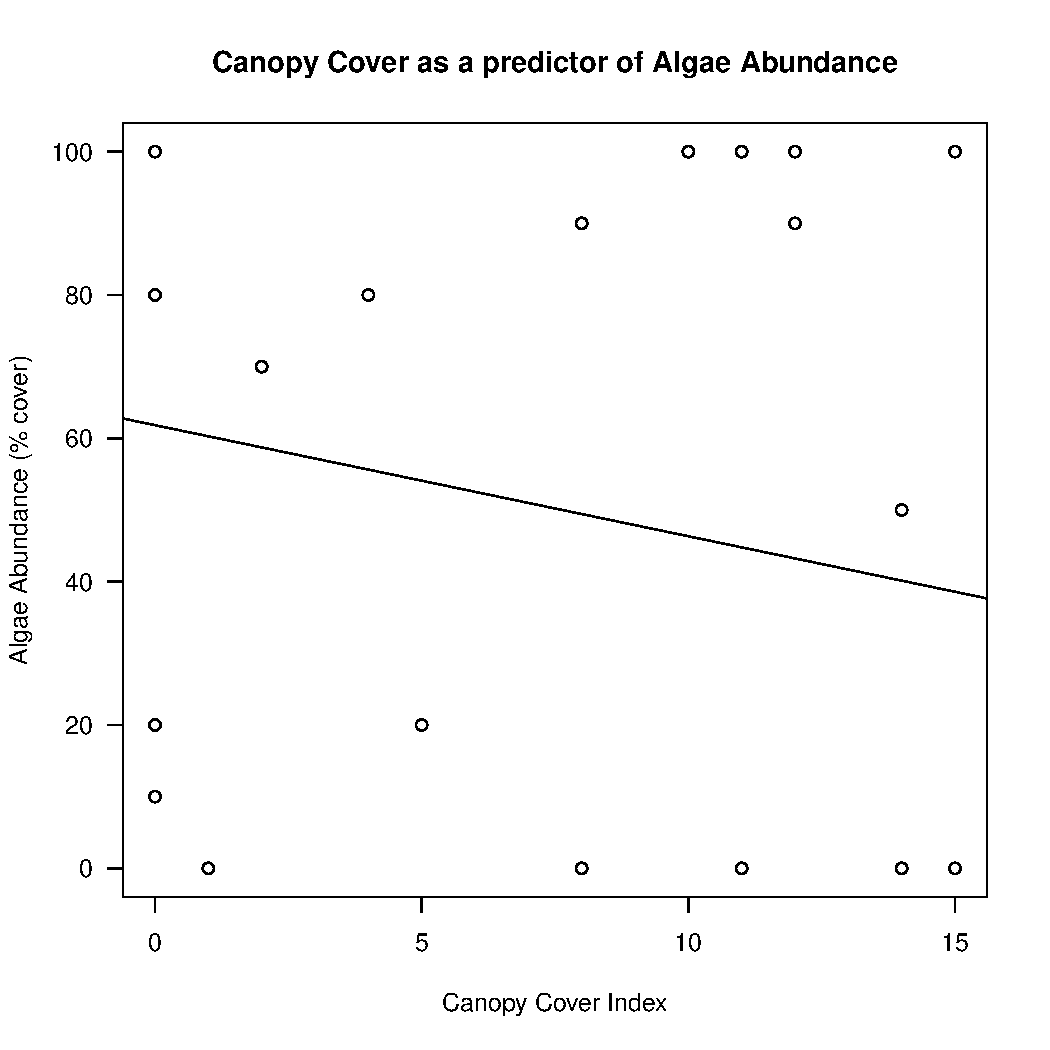
\includegraphics[width=\maxwidth]{figure/unnamed-chunk-4-1} 

\end{knitrout}
Bed composition did have a stronger relationship with Alage Abanundance, as shown in the figure above. 0 = fine sediment, while 1 = coarse sediment. Our P value=0.0643 which means we cannot reject null hypothesis, but only barely. This indicates that there is probably some relationship between algae cover and sediment composition of the stream bed, and this should be examined in future. In general, alage seem to perhaps prefer coarser sediment. 

\begin{knitrout}
\definecolor{shadecolor}{rgb}{0.969, 0.969, 0.969}\color{fgcolor}\begin{kframe}
\begin{alltt}
\hlkwd{boxplot}\hlstd{(Algae}\hlopt{~}\hlstd{Site_new,importupdated,} \hlkwc{ylab}\hlstd{=}\hlstr{"Algae Abundance (% cover)"}\hlstd{,}\hlkwc{xlab}\hlstd{=}\hlstr{"Site name"}\hlstd{,}\hlkwc{main} \hlstd{=}\hlstr{"Reach Site as a predictor of Algae Abundance"}\hlstd{,}\hlkwc{las}\hlstd{=}\hlnum{1}\hlstd{)}
\end{alltt}
\end{kframe}
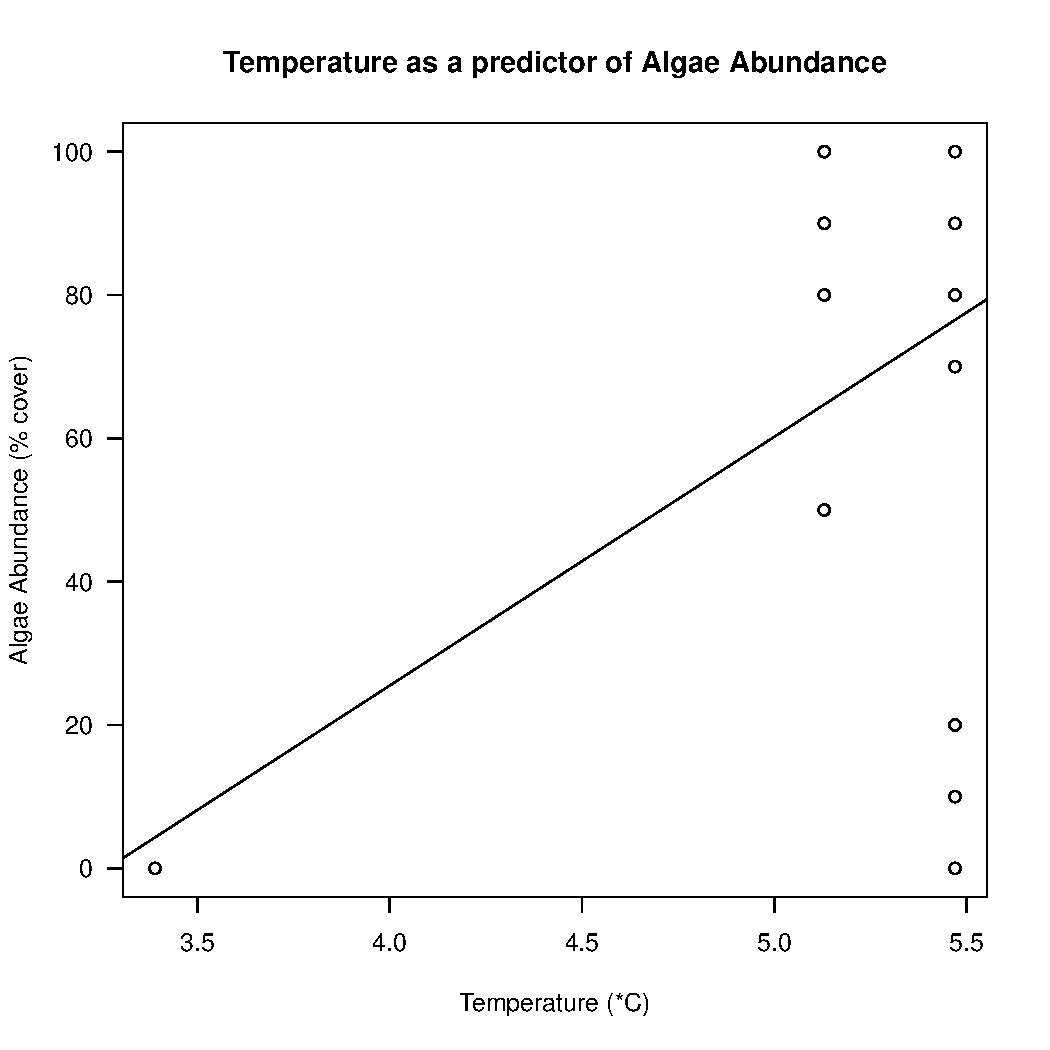
\includegraphics[width=\maxwidth]{figure/unnamed-chunk-5-1} 

\end{knitrout}
As a control, we also analyzed to what extend Reach Site alone could predict Algae Abundance. Our ANOVA test yielded p-value: 0.008176 which means the reach of the river studied is alone one of our best predictors of algae abundance, second only to temperature variation. However, our temperature variation data was merged with our algae data after the fact, and for each site, all measurements were assigned the same temp\_range value. Therefore, the high predictive value of temp\_range could be just an artifact of that methodological decision. However, temperature variations p-value was over 2 orders of magnitude smaller than Reach Site alone (3.49e-05 vs. 8.17e-03 respectively), so it remains thoroughly plausible that water temperature variation is predictor of algae abundance independent of site variation. Because of our experiemental design, it is unfortunately impossible to control by site for temperature variation and see if the relationship remains robust. This should be examined in future work. We counted an average of 20.133 suckers in the morning with a standard deviation of 6.007 fish.  In the afternoon, we counted an average of 32.25 with a standard deviation of 9.928, meaning both the average and the variance were higher in the afternoon.  The river was 27.764°C in the morning and increased to 28.456°C in the afternoon.  We calculated a p-value of 6.027e-13, which is less than .05 so we can reject our null hypothesis that tie of day will have no effect on the number of fish.
\begin{knitrout}
\definecolor{shadecolor}{rgb}{0.969, 0.969, 0.969}\color{fgcolor}\begin{kframe}
\begin{alltt}
\hlstd{newmetadata} \hlkwb{<-} \hlkwd{read.csv}\hlstd{(}\hlstr{"/home/CAMPUS/cmfa2015/Santa Ana Sucker/Data/Data_Tues_2/newmetadata.csv"}\hlstd{)}
\end{alltt}
\end{kframe}
\end{knitrout}
\begin{knitrout}
\definecolor{shadecolor}{rgb}{0.969, 0.969, 0.969}\color{fgcolor}\begin{kframe}
\begin{alltt}
\hlkwd{boxplot}\hlstd{(Fish}\hlopt{~}\hlstd{Section,newmetadata,} \hlkwc{ylab}\hlstd{=}\hlstr{"Fish"}\hlstd{,}\hlkwc{xlab}\hlstd{=}\hlstr{"Time of Day"}\hlstd{,}\hlkwc{main} \hlstd{=}\hlstr{"Time of Day as a predictor of Fish"}\hlstd{,}\hlkwc{las}\hlstd{=}\hlnum{1}\hlstd{)}
\end{alltt}
\end{kframe}
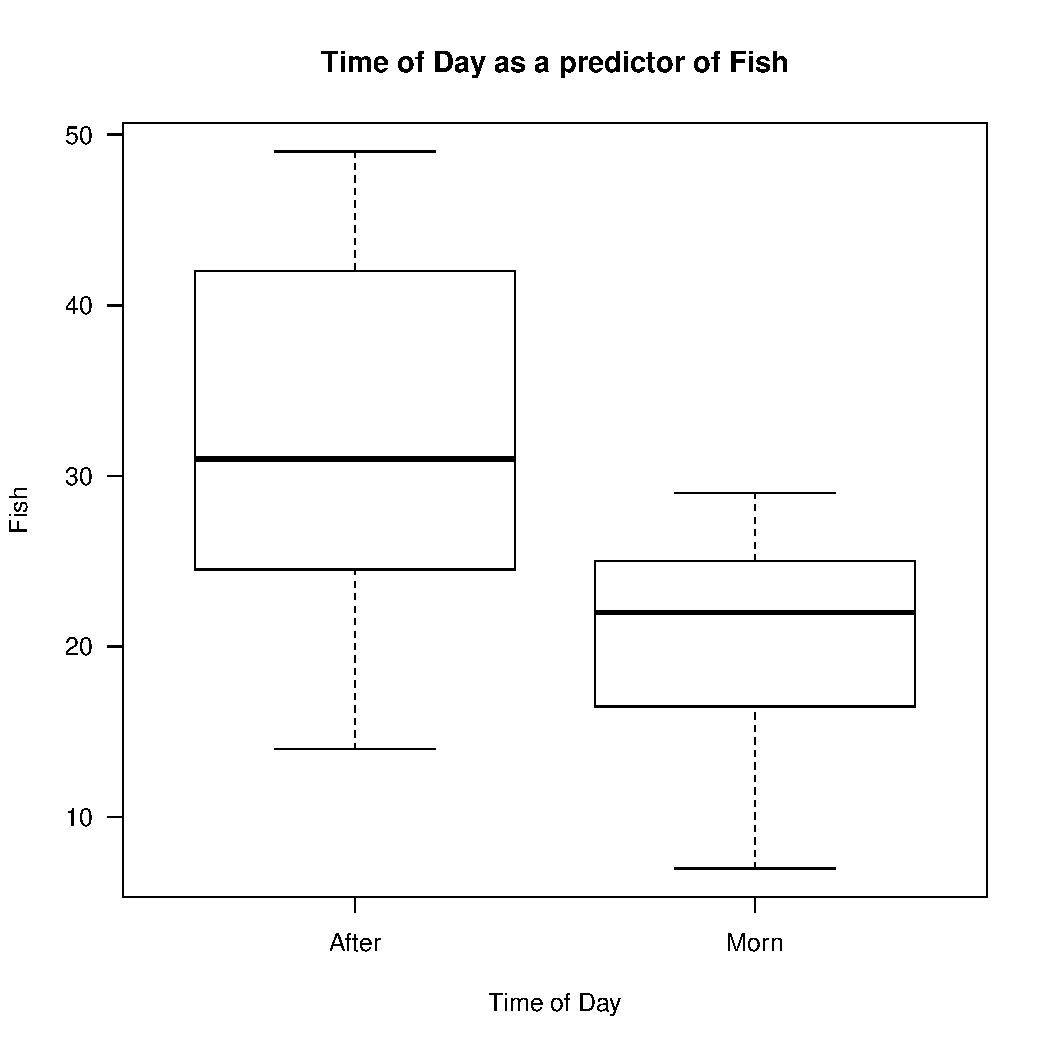
\includegraphics[width=\maxwidth]{figure/unnamed-chunk-7-1} 

\end{knitrout}
\begin{tabular}{ |p{1.5cm}||p{1cm}|p{1cm}|{p2cm}|{p2cm}|{p2cm}|{p2cm}|{p2cm}|  }
 \hline
 \multicolumn{8}{|c|}{Videography Summary Statistics} \\
 \hline
 Section & Min & Max & Mean & Median & 1st Quartile & 3rd Quartile & K\\
 \hline
 Morning & 7 & 29 & 20.13 & 22  & 16.75 & 25 & -0.6\\
 Afternoon & 14 & 49 & 32.25 & 31 & 24.75 &  42 & -1.3\\
 \hline
\end{tabular}



\section{Discussion}


Certain issues we ran into during our study included visibility and camera placement. Unfortunately, we did not formulate a standardized method with which to place our cameras in the water. For this reason, there were differences in footage from morning to afternoon as well as from site to site. For future studies, we recommend including physical place-markers in the river for the cinderblock structures, maybe in the form of flags placed directly in the river bed. Markers inside of the cinderblock structure that delineate the exact position and angle of the cameras would also be ideal in order to ensure the same exact field of vision is present throughout the collected footage. Additionally, a marker such as a graphic scale would be useful to have in the camera’s field of vision in order to figure out size of the fish and distance from the camera. Finally, our model of GoPro did not have a timestamp feature. Though we were able to figure out the initial recording times from the data saved in each individual video file, a timestamp would have greatly facilitated and ensured the accuracy of our counting process.

For future studies of this sort, a longer data sampling process would be ideal. While we were only able to collect and analyze one hour of footage each for the morning and afternoon sections, a more robust study might have 20 or so hours each over the course of a single month, or even a lot more than this, as there is no limit to the amount of data that could be taken for this study due to changes in season, water influx differences, and other factors.


Our results were skewed due to several hiccups that occurred throughout the process of our experiment. The first time we collected our samples, said samples were not processed on the same day as collection. 
We don’t have the initial BOD measurements and so our group had to think outside of the box and backpedal some in order to work backwards and acquire the numbers needed in order to make the vital calculations and check our work.
When in the middle of checking the BOD of our samples after the 5 day incubation period we realized that we had not turned on the motor for the previous handful of samples as well as some in our initial stages. In order to accommodate this discrepancy, we decided to include spin v no spin as apart of our variables in our project to see the results we would get since there was such a huge margin between the numbers when the solutions were stirred and when they were not.
In order to fill any gaps in our own research and numbers, we have also decided that it would be best that we correlate our results with those collected by the Fish and Wildlife service when they conducted their electroshock tests on the fish. 


Future experiments can improve upon our methods by using the optimum amount of source water and dilution water to get the optimum about of BOD depletion. The ideal BOD depletion reading was given at 25 mL of source water and 275 mL dilution water. It would also be best if it is meticulously made sure of that the BOD is taken of the initial samples. Important to the process is to have every sample spun each time to allow for consistency and as much accuracy as possible with each BOD reading. 

Our videos of site 2 contained so few fish that we were unable to draw any conclusions from the data.  In the morning there were no Santa Ana suckers seen in the entire hour, and in the afternoon there was one sucker that would occasionally swim out from behind a rock.  This could be because the temperature that far upstream was too hot for the suckers to live there; the temperature data found that at that location the water was around 29°C in the afternoon and 25°C in the morning.  It is also possible that our camera was placed in a section of the river that the suckers don’t like, so the lack of fish could have had nothing to do with temperature.
When we compared the number of fish downstream in the afternoon compared to the morning, we had a p-value of 6.027e-13, meaning there were significantly more suckers in the afternoon than there were in the morning.  This suggests that the suckers do move downstream throughout the day to get to cooler temperatures.  On the afternoon we tested, the plunge pool (downstream) was 28.5°C, whereas the river at our upstream location, closer to the concrete, was 29.4°C.  However, we cannot definitively prove that we observed more fish in the afternoon because of the temperature change; there could have been a variety of other factors.  For example, the fish could have moved from one river bank to the other throughout the day to stay in the shade of the brush as the sun moved.

\section{Conclusion and Recommendations}


\section{Literature Cited}

\bibliographystyle{apalike}
\bibliography{report}

Greenfield, D. W., Ross, S. T., \& Deckert, G. D. (1970). Some aspects of the life history of the Santa Ana sucker, Catostomus (Pantosteus) santaanae (Snyder). Calif. Fish Game, 56(3), 166-179. 



\section{Appendix: Detailed Methods}

To set up the cameras, we removed them from the packaging, inserted a microSD card into each, and charged them fully by connecting the included USB cables to a computer. The cameras needed to be fully charged before we were able to adjust the settings. Once the cameras were sufficiently charged, we set the filming settings to record in 720p x 30fps. We set the cameras aside and left them charging. 

Next, we charged all four of the waterproof Re-Fuel battery packs. As these were charging, we put together our cinder block mounting structures. We took our cinder block cubes and set them up on a clean, stable table. We connected the flat adhesive mounts that were included with the GoPros and connected a GoPro camera to each. Since the cinder blocks were open on two parallel sides, we were able to see right through the cinder block cube to the other side. One of us stood on one side with the GoPro and mount, and the other stood on the other side of the opening. One of us turned the GoPro on and put the camera with the mount inside the cinder block cube, using the view on the screen to find the best position for the mount inside of the cube, taking care to ensure we could clearly see the other person on the other side. We found an ideal place where the view was mostly unobstructed by the sides of the cube but the cameras were still far enough inside the cube that they wouldn’t be too easily spotted by passersby. This spot was 5 cm from the edge of the cube. We traced the front and the back of the mount so we could glue it in the correct place. We repeated this procedure for the second cube and mount, and standardized the construction by placing the mount in the second cube 5 cm away from the edge of the cube. 

In order to securely glue the mount in place, we used Gorilla glue. To activate the Gorilla glue, we first had to moisten one of the surfaces with water. We moistened the mounts on the adhesive side. We did not remove the adhesive backing so we could reutilize the mounts in the future. Once the mount was damp, we put Gorilla glue on the cinder block inside the lines we had drawn around the mount. We then placed the mount on the Gorilla glue, taking care to align the edges of the mount with the lines we had drawn. Next, as per the Gorilla glue instructions, we found a heavy object that could provide significant pressure on the mount and that would fit inside the cube. We left this for three hours to harden.

Upon returning to the lab, we removed the heavy objects from the cube and checked the seal on the mount and cinder block to ensure the bond had successfully cemented. After this, we went to work on attaching the cinder block backs to close up one of the open sides on the cubes. We repeated much of the same process we used when attaching the mounts to the cubes, and followed the Gorilla Glue instructions carefully. First, one of us moistened the cinder block back while the other applied Gorilla Glue to the edge of the cube. Then, we carefully aligned the corners of the back with the cube. We repeated this with the second cube. Seeing that the cinderblock back was heavy enough on it’s own, we did not place a heavy object on top of this structure and instead simply left it to dry and harden overnight.

Finally, we checked on the cameras and battery packs again to ensure they had charged. We left them plugged in overnight. We also packed away the Gorilla Glue, the multiple SD cards, paper towels, and extra mounts in a field kit so we could deal with any emergencies in the field.

We started our first recording session at 10 am.  We drove to the downstream site and found a spot under brush cover in a pool next to a fast moving section of the stream.  We first placed the cinderblock squarely on the riverbed and positioned it facing the fast moving water.  We then turned the camera on, pressed record, and placed it on the mount in the cinderblock.  We let it run for a few seconds, then took it out and watched the video to ensure it was recording at a good angle.  We then pressed record again and replaced it.  Before leaving, we marked the area with flags so we would be able to find it again.
Next, we walked approximately 20 minutes upstream to another covered pool next to a fast moving section, and repeated the camera placement procedures.  We marked with flags, and then left.

We returned at approximately 2 pm.  We took out the camera at the downstream site, replaced the memory card and the battery pack, hit record, and replaced the camera exactly as it was positioned previously.  We then walked upstream and did the same thing with the second camera.  After returning, we cleared the memory cards and plugged in the battery packs.
Our last recording session was at 8 am the next morning.  We replaced the memory cards and battery packs again and returned the cameras to their positions.  One of us returned the next day to collect the cameras.

\section{Conclusion and Recommendations}
There is a statistically significant variation of algae abundance between the 3 sites examined in our study. Some measurements showed up to 100 percent algae cover, while others exhibited none. This variation suggests the possibility that algae may be controlled by specific variables. We tested whether water temperature, water temperature variation, canopy cover, or stream bed composition could explain these variations. Of these possible causal factors, we found the strongest evidence for higher water temperature variation exerting a positive effect of algae abundance. The relationship between algae cover and streambed sediment composition of the stream bed was not statistically significant at the 95 percent level, but did tentatively suggest that algae may prefer coarse sediment. Red Algae in the Santa Ana River has a highly unequal distribution, that appears to be controlled in part by water temperature variation, with a possible small contribution of streambed sediment composition. 
Our exploratory study is one of the first to examine what variables may control red algae's distribution in the Santa Ana River. While the limited scope of this research eliminated the possibility of conclusive findings, we can suggest promising areas for further research. Future studies should more systematically examine the relationship between temporal variability in water temperature and algae abundance. Sediment type should be assigned to narrow categories such as silt, sand, gravel, and cobbles rather than simply being tagged as fine or coarse. More than 3 reaches/sites should be used. Most importantly, red algae’s co-occurrence with the federally endangered Santa Ana sucker should be examined. These improvements on our experiment will yield a much better idea of what factors control red algae’s distribution in the Santa Ana River, and create a statistically supported foundation for considering the algae’s effect on Santa Ana Suckers. 


\end{document}
